\chapter{Literature Review}
\label{chap:2}
\section{Nuclear Fuel Cycle Simulator History}
The nuclear fuel cycle represents the nuclear fuel life cycle from initial
extraction through processing, use in reactors, and, eventually, 
final disposal.
This complex system of facilities and mass flows 
collectively provide nuclear energy 
in the form of electricity \cite{yacout_modeling_2005}.
A closed nuclear fuel cycle reprocesses used fuel, whereas an open 
nuclear fuel cycle does not.  
The US has an open nuclear fuel cycle; other countries, such as France, 
have a closed nuclear fuel cycle. 

% Why were nuclear fuel cycle simulators introduced 
Nuclear fuel cycle system analysis tools were introduced to investigate 
nuclear fuel cycle dynamics at a local and global level. 
Nuclear fuel cycle simulators' primary purpose   
is to understand the dependence between various system designs, deployment 
strategies, and technology choices
in the nuclear fuel cycle and the impact their variations have on 
the system's performance. 
Nuclear fuel cycle simulator results are used to guide research 
efforts, advise future design choices, and provide 
decision-makers with a transparent tool for evaluating \gls{FCO} 
to inform big-picture policy decisions \cite{yacout_modeling_2005}.
Nuclear fuel cycle simulators were initially introduced 
by the Nuclear Strategy Project at Science Applications International Corp 
to provide simple system dynamic models to improve technical dialog between 
policymakers and expert groups \cite{yacout_modeling_2005}.
Since then, national laboratories around the globe have driven 
development of nuclear fuel cycle simulators. 
These simulators track the flow of materials through the nuclear fuel cycle, 
from enrichment to final disposal of the fuel. 
However many have been developed for customized applications, resulting in 
inflexible architectures \cite{huff_fundamental_2016}.  

Two methods can be used to model facility and material flow in 
nuclear fuel cycle simulators: fleet-level and agent-level.  
Fleet-based models do not distinguish between discrete facilities 
or materials but instead lump them into fleets and streams but they 
offer simplicity and lower computational cost. 
Agent-based models treat facilities and materials as discrete 
objects. 
This method's advantages are more flexible simulation control,
ease of simulating a wide range of scenarios with new 
technologies, enabling of plug-and-play comparison of modeling 
methodologies, and allowing for a range of fidelities.  
Many nuclear fuel cycle simulators value integral effects over isotopic and 
facility-level resolution by modeling only fleet-level dynamics,
grouping facilities into fleets and materials into streams \cite{huff_fundamental_2016}.

Historically, national laboratories have restricted public access to their tools, 
resulting in universities and 
other non-laboratory organizations creating their 
own nuclear fuel cycle simulator tools. 
Table \ref{tab:nfctools} shows a breakdown of all major nuclear fuel cycle simulators
and the organization(s) associated with them.  

\begin{table}[]
    \caption{Nuclear fuel cycle simulator tools and their corresponding organizations.}
    \label{tab:nfctools}
    \centering
    \doublespacing
    \small
    \resizebox{1\textwidth}{!}{
    \begin{tabular}{lll}
    \hline
    \textbf{NFC Simulator} & \textbf{Country} &\textbf{Organization(s) associated with it}                                    \\ \hline
    ANICCA \cite{skarbeli_quantification_2020}& Belgium & \gls{SCK CEN}\\
    CAFCA \cite{guerin_impact_2009} & USA &\gls{MIT} \\
    CLASS  \cite{mouginot_class_2012}          &France                      &  \gls{CNRS}, \\ && \gls{IRSN}                                    \\
    COSI   \cite{coquelet-pascal_cosi6:_2015}        &France                        &   \gls{CEA}                    \\ 
    \Cyclus \cite{huff_fundamental_2016}              & USA  & \gls{UW}, \\ && \gls{UIUC} \\ 
    DESAE  \cite{tsibulskiy_desae_2006} &-& \gls{OECD} \\ 
    DYMOND \cite{yacout_modeling_2005}   &USA                             & \gls{ANL}                                                                                               \\ 
    EVOLCODE2 \cite{alvarez-velarde_evolcode2_2007} & Spain &\gls{CIEMAT}\\ 
    FAMILY21 \cite{mccarthy_benchmark_2012} & Japan&\gls{JAEA} \\ 
    MARKAL \cite{fishbone_markal_1981} & USA & \gls{BNL} \\
    NFCSim \cite{schneider_nfcsim:_2005}& USA &\gls{LANL} \\
    NFCSS \cite{iaea_nuclear_2007}& -&\gls{IAEA} \\
    ORION  \cite{gregg_analysis_2012}      & UK                          & \gls{NNL}                                                                                             \\ 
    VISION \cite{jacobson_vision:_2006}      & USA                          & \gls{INL}                                                                                               \\  \hline
    \end{tabular}}
    \end{table}

In this work, we use the \Cyclus and DYMOND nuclear fuel cycle simulator tools. 
The \Cyclus nuclear fuel cycle simulator was created to break the practice of 
tools with inflexible architectures and restricted access \cite{huff_fundamental_2016}.
\Cyclus is an open source nuclear fuel cycle simulator with agent-based 
modeling of discrete facilities and isotopic materials. 
With an agent-based framework, the simulator tracks transformation and 
trade of resources between agents with customizable behavior
\cite{huff_fundamental_2016}. 
This enables extension and reuse of this tool for fuel cycle 
simulations with different objectives. 
DYMOND is a hybrid nuclear fuel cycle simulator tool that uses fleet-based 
modeling for all facilities and materials 
with an exception of discrete modeling for reactor facilities. 
Chapter \ref{chap:3} provides more detail about \Cyclus and DYMOND. 

\section{Transition Scenario Capabilities in Nuclear Fuel Cycle Simulators}
\label{sec:egs}
The Office of Nuclear Energy's
\gls{FCO} Campaign led an evaluation 
and screening study of a comprehensive set of nuclear \glspl{FCO} 
to identify \glspl{FCO} with the potential to substantially 
improve the nuclear fuel cycle in the challenge areas
\cite{wigeland_nuclear_2014}. 
The evaluation and screening study identified 40 
\glspl{EG} to represent a comprehensive set of 
all possible nuclear fuel cycles \cite{wigeland_nuclear_2014}. 
Each evaluation group consists of a group nuclear fuel cycles that
similar resource requirements, fuel mass usage and compositions, 
and disposal needs \cite{wigeland_nuclear_2014}. 
The study assessed each evaluation group using 
9 evaluation criteria: nuclear waste management, 
proliferation risk, nuclear material security risk, 
safety, environmental impact, resource utilization, 
development and deployment risk, institutional issues, and 
financial risk.  
The study concluded that fuel cycles
involving continuous recycling of co-extracted U/Pu or U/TRU in 
fast spectrum critical reactors consistently scored high overall 
performance.
EG23, EG24, EG29, and EG30 are the high-performing fuel cycle options
\cite{wigeland_nuclear_2014}.
These evaluation groups were evaluated at an equilibrium state to 
understand their end-state benefits.
Knowing the most promising end-state evaluation groups,
the next step is to evaluate and compare the transition process 
from the current EG01 
state to these promising evaluation groups \cite{feng_standardized_2016}. 

The transition from the once-through fuel cycle to a closed fuel cycle 
has a slow dynamic, and a complex interdependence of many factors. 
Thus, the study of transition scenarios using a nuclear fuel cycle simulator 
is key to understanding the influence of these multi-coupled factors on the transition. 
The U.S. national laboratories conducted a benchmarking effort
of transition scenario capabilities in nuclear fuel cycle simulators
\cite{feng_standardized_2016,guerin_benchmark_2009}. 
This comparison study aims to drive nuclear fuel cycle simulator advancements and build 
confidence in the use of nuclear fuel cycle simulators in 
strategic and policy decisions \cite{feng_standardized_2016}. 

Both nuclear fuel cycle simulator tools used in this thesis, \Cyclus and DYMOND,
were verified in a transition scenario benchmarking effort
\cite{feng_standardized_2016,bae_standardized_2019}.
The reference problem used in the benchmark was a simplified 
transition from a one hundred 1000-MWe \glspl{LWR} to a 
333.3-MWe \gls{SFR} fleet. 
They were found to have excellent agreement with the 
analytical solution and other nuclear fuel cycle simulators, 
ORION, VISION, and MARKAL.  
This benchmarking effort proved that these nuclear fuel cycle simulators
are capable of simulating a simple transition scenario. 
However, to evaluate the nuclear fuel cycle simulators' flexibility, 
Feng et al concluded that more efforts must be made to model realistic transition scenarios
\cite{feng_standardized_2016}.

\section{Sensitivity Analysis Studies}

% sensitivity analysis in dynamic simulations in other fields  

We simulate transition scenarios to predict the future; 
however, when implemented in the real world, the simulated 
scenarios tend to deviate from the optimal scenario.
Also, transition scenario analysis using nuclear fuel cycle simulators 
are imperfect representations of the real world \cite{noauthor_effects_2017}.
Therefore, sensitivity analysis studies of nuclear fuel cycle transition 
scenarios must be conducted to better understand the impact of the variation 
of input parameters on performance metrics, enabling the nuclear fuel cycle simulators to
more reliably inform policy decisions \cite{passerini_systematic_2014}. 

Transition scenario sensitivity analysis is a technique used to determine how varying
different input variables impacts a transition scenario's performance metrics.
Assumptions about facility parameters and technology readiness 
are made when setting up the simulation scenarios. 
Sensitivity analysis evaluates each performance metric's 
sensitivity to each assumption. 
Previous work towards sensitivity analysis and uncertainty quantification of 
nuclear fuel cycle simulations used these terms interchangeably
because uncertainty quantification is viewed as design uncertainty \cite{noauthor_effects_2017}.
For example, a never-been-built pyrochemical reprocessing 
facility's throughput is viewed as a variable design parameter.
We determine how variation of the pyroprocessing 
facility's throughput impacts performance metrics.
Therefore, in this thesis, we refer to both sensitivity analysis 
and uncertainty quantification as sensitivity analysis. 
By conducting studies on an extensive input parameter set, 
it is possible to determine the input parameters' that each performance 
metric is most sensitive to.
This helps us target where we should conduct closer 
sensitivity analysis and add further modeling detail.
It also identifies which parameters the system is relatively 
insensitive to \cite{noauthor_effects_2017}. 

In this work, we use three types of sensitivity analysis: 
one-at-a-time, synergistic, and global.

\subsection{One-at-a-time Sensitivity Analysis}
The one-at-a-time sensitivity analysis technique estimates 
the isolated effect of one input variable. 
This approach gives each variable's local impact 
on the performance metrics. 
\gls{OECD} conducted an one-at-a-time sensitivity analysis \cite{noauthor_effects_2017} 
on key nuclear fuel cycle input parameters
and quantified the impacts on the performance metrics. 
In the OECD study, the base scenario used has a duration of 200 years and begins 
with \glspl{PWR}, that transition to \glspl{SFR} while 
maintaining constant electricity production. 
Each parameter was varied independently for three cases: 
the base case, a high case, and a low case with respect to the base case. 
The results of these variations on the performance metrics 
are expressed in tornado plots and sensitivity tables. 
The OECD study's analysis overview is given in Figure \ref{fig:oecd-sensitivitytable}. 
Figure \ref{fig:oecd-tornado} shows an example tornado plot 
from the OECD study that represents 
the sensitivity of the separated Pu in storage amount to the 
various input parameters. 

\begin{figure}[]
	\begin{center}
		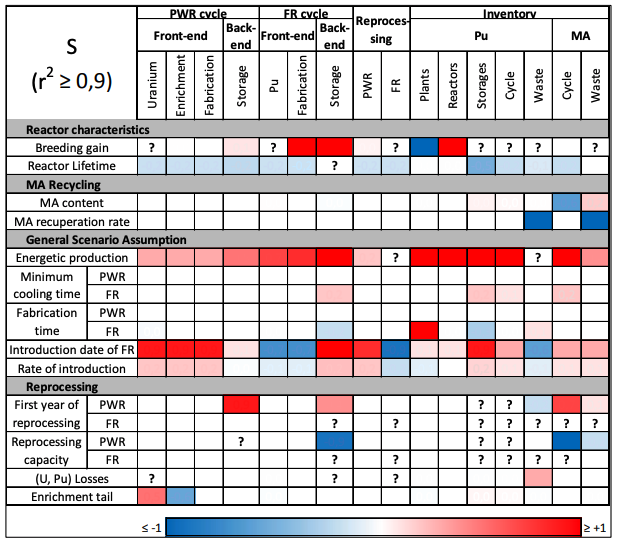
\includegraphics[scale=0.75]{./figures/oecd-sensitivitytable.png}
	\end{center}	
        \caption{Overall results from OECD one-at-a-time sensitivity analysis 
        study. This is reproduced from the OECD report \cite{noauthor_effects_2017}.
        Sensitivity Table with an overview of all the sensitivity indicators 
        “S” obtained from the various input
        parameters (one row for each input parameter) and the various output parameters (one
        column for each output parameter). When a sensitivity coefficient is positive (red), this means an increase 
        of the input parameter induces an increase of the output parameter. Whereas, when it is blue, 
        this means an increase of the input parameter induces a decrease of the output parameter.
        When a coefficient of determination $r^2$ is lower than 0.9, then the related sensitivity
        indicator is replaced by a question mark “?” in the table.
        When the output parameter is not impacted by the variation of the input parameter, then
        the related sensitivity indicator is not available and it is replaced by a blank in the table.
        \cite{noauthor_effects_2017}.
        }
	\label{fig:oecd-sensitivitytable}
\end{figure}

\begin{figure}[]
	\begin{center}
		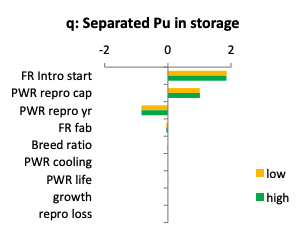
\includegraphics[scale=1]{./figures/oecd-tornado.png}
	\end{center}	
		\caption{A tornado plot from the OECD one-at-a-time sensitivity analysis 
        study, showing the sensitivity of the separated Pu in 
        storage amount to each input parameter. This is 
        reproduced from the OECD report \cite{noauthor_effects_2017}.}
	\label{fig:oecd-tornado}
\end{figure}

\subsection{Synergistic Sensitivity Analysis}
\label{sec:syn}
The synergistic sensitivity analysis technique involves multi-parameter 
input sweeps to view how synergistically changing input variables 
impacts the performance metrics.  
Synergistic sensitivity analysis is conducted by varying 
two input variables simultaneously and viewing their 
combined impact on each performance metric or a combination 
of weighted performance metrics. 
Passerini et al \cite{passerini_systematic_2014} applied
this analysis method on nuclear fuel cycle simulations. 
Figure \ref{fig:passerini_payoff} shows the results of a synergistic analysis 
conducted by Passerini et al \cite{passerini_systematic_2014} 
in which thermal reprocessing and fast reactor technology 
introduction dates were varied. 
The plot shows an objective payoff surface representing a combination of 
weighted optimization criteria: minimize construction of reprocessing plants, 
minimize \gls{LCOE}, minimize depleted uranium generated, and minimize total SWU used.
This type of synergistic studies successfully informs on how variation in 
two input variables impacts the system; however, if more than two input variables 
are varied, it is difficult to visualize the impact on the system in a plot. 
Therefore, the subsequent section's global sensitivity analysis method is introduced to 
inform on the global sensitivity of the system. 

\begin{figure}[]
	\begin{center}
		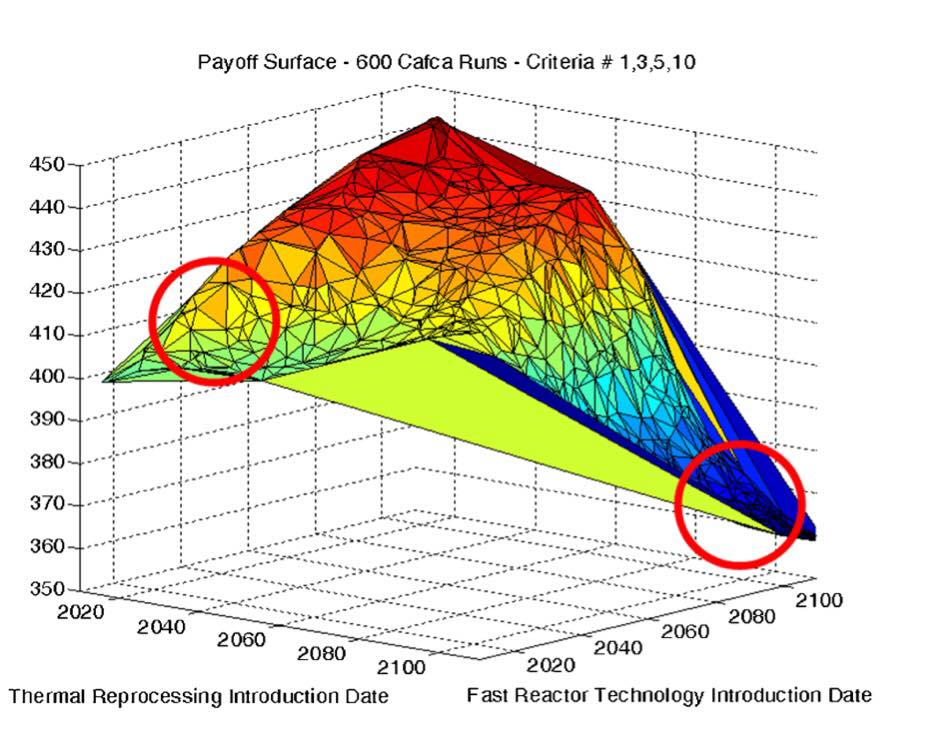
\includegraphics[scale=0.45]{./figures/passerini_payoff.jpg}
	\end{center}	
		\caption{Payoff surface for variation in thermal 
		reprocessing and fast reactor technology introduction date
        \cite{passerini_systematic_2014}. The payoff surface represents
        a combination of weighted optimization criteria: minimize construction of reprocessing plants, 
        minimize \gls{LCOE}, minimize depleted uranium generated, and minimize total SWU used. 
        }
	\label{fig:passerini_payoff}
\end{figure} 

\subsection{Global Sensitivity Analysis}
\label{sec:sobol}
To fully consider the synergistic effects of
simultaneous variation of all the nuclear fuel cycle input parameters, 
a variance-based approach can be used instead \cite{thiolliere_methodology_2018}.
Thiolliere et al. conducted a global sensitivity analysis of a 
nuclear fuel cycle transition scenario by using Latin Hypercube sampling
\cite{sobol_global_2001} to generate Sobol indices \cite{mckay_comparison_2000}
that indicate which design parameters have 
the most influence on the performance metrics.  
They applied this method to a simplified PWR UOX and PWR MOX fleet. 
Latin Hypercube sampling is a statistical method for generating random samples of 
parameter values from a multidimensional distribution. 
For Latin Hypercube Sampling of M input parameters, the user first chooses the  
number of sample points, N, 
then each parameter's input space is divided into N sub-sections. 
The algorithm will then select a random value from each sub-section for each input 
parameter. 
Once there is a list of samples for each input parameter, they are combined randomly 
to form M-dimensional sets \cite{sobol_global_2001}.
The nuclear fuel cycle simulation is run M times and the performance metrics of interest are recorded. 
Sobol sensitivity analysis provides how much variability in the model's 
performance metrics is dependent on each input parameter \cite{zhang_sobol_2015}. 
Sobol Indices decomposes the 
variance of the metric into fractions attributed to inputs or sets of inputs.
A large Sobol index signifies that variation in that input 
variable is more impactful to the output parameter. 
A model is viewed as a function: 
\begin{align*}
    Y &= f(\textbf{X})
    \intertext{where:}
    Y &= \mbox{Performance metric} \nonumber\\ 
    \textbf{X} &= \mbox{vector of \textit{d} input parameters} \nonumber \\
    d &= \mbox{No. of varying input parameters} \nonumber
\end{align*}
First order Sobol indices measure the effect of one input parameter on 
the performance metric with an average over variations in other input 
parameters \cite{im_sensitivity_1993}: 
\begin{align*}
    S_i &= \frac{V_i}{Var(Y)}
    \intertext{where:}
    S_i &= \mbox{First order sensitivity index} \nonumber \\
    V_i &= Var_{X_i}(E_{\textbf{X}(\sim i)}(Y|X_i)) = \mbox{Conditional variance} \nonumber \\
    \textbf{X}(\sim i) &= \mbox{the set of all variables except $X_i$}
\end{align*}
Total-effect Sobol indices measure the effect of the first order Sobol index plus all the 
interactions the one input parameter has with other input parameters \cite{homma_importance_1996}: 
\begin{align*}
    S_{Ti} &= 1-Var_{\textbf{X}(\sim i)}(E_{X_i}(Y|\textbf{X}(\sim i)))
\end{align*}


\subsection{Summary of Sensitivity Analysis Studies}
Sensitivity analysis studies of nuclear fuel cycles have previously been used to narrow 
down and compare a wide range of nuclear fuel cycle scenarios to determine 
the ideal scenario. 
The evaluation and screening study \cite{wigeland_nuclear_2014} determined that the desired 
fuel cycle end states were fuel cycles
involving continuous recycling of co-extracted U/Pu or U/TRU in 
fast spectrum critical reactors.
These evaluation and screening study's sensitivity analysis focused on macro-level input 
parameters such as types of reactor and reprocessing technologies.
However, sensitivity analyses regarding dynamic nuclear fuel cycle transitions are rare. 
The only relevant sensitivity study was conducted by OECD 
\cite{noauthor_effects_2017}, however it was a basic one-at-a-time 
sensitivity analysis.   
Therefore, synergistic and global sensitivity analysis studies focused on
micro-level input parameters such as length of cooling time and  
introduction date of reprocessing/reactor 
technologies, should be conducted to 
understand how their variation impacts the performance metrics. 
Using the sensitivity analysis results, these transition scenarios can be 
further optimized and used to inform other nuclear research areas. 
For example, by studying how the throughput of a reprocessing facility impacts the 
performance metrics, we can determine the ideal reprocessing facility size. 